\documentclass[11pt,a4paper]{article}
\usepackage{amsmath}
\usepackage{amsthm}
\usepackage{amssymb}
\usepackage[margin=2cm]{geometry}
%\usepackage{thmbox}
\usepackage{graphicx}
\usepackage[dvipsnames,usenames]{color}
\usepackage{url}
\usepackage{comment}
\usepackage{amsmath, amsthm, amssymb,enumerate}

%\usepackage{enumerate}
%\usepackage{titlesec}
%\usepackage{Rvector}
%\usepackage{mathabx}
\newcommand{\qrq}{\quad\Rightarrow\quad}
\newcommand{\qarq}{\quad&\Rightarrow\quad}
\newcommand{\alp}{\alpha}
\newcommand{\claim}{{\underline{\it Claim:}}~~}
\newcommand{\dbR}{\mathbb{R}}
\newcommand{\ndimr}{\mathbb{R}^n}
\newcommand{\vare}{\varepsilon}
\newcommand{\since}{\because\;}
\newcommand{\hence}{\therefore\;}
\newcommand{\en}{\par\noindent}
\newcommand{\fn}{\footnotesize}

\newcommand{\sect}[2]{#1~~{\mdseries\tiny(#2)}}

\renewcommand{\(}{\left(}
\renewcommand{\)}{\right)}

\let \ds=\displaystyle

\usepackage{xeCJK}
\setCJKmainfont[AutoFakeBold=5,AutoFakeSlant=.4]{標楷體}

%\usepackage{fancyhdr}
%\pagestyle{fancy}
%\renewcommand{\headrulewidth}{0pt}

\renewcommand{\thesection}{Lecture \arabic{section}}
\renewcommand{\thesubsection}{\Roman{subsection}}

\usepackage[T1]{fontenc}

%%%% F U N C T I O N %%%%%
\newcommand{\abs}[1]{\left|#1\right|}
\newcommand{\norm}[1]{\left\|#1\right\|}
\newcommand{\inn}[1]{\left<#1\right>}
\newcommand{\f}[1]{f\!\left(#1\right)}
\newcommand{\g}[1]{g\!\left(#1\right)}
\newcommand{\h}[1]{h\!\left(#1\right)}
\newcommand{\x}[1]{x\!\left(#1\right)}
\newcommand{\D}[1]{D\!\left(#1\right)}
\newcommand{\N}[1]{N\!\left(#1\right)}
\renewcommand{\P}[1]{P\!\left(#1\right)}
\newcommand{\R}[1]{R\!\left(#1\right)}
\newcommand{\V}[1]{V\!\left(#1\right)}
\newcommand{\function}[2]{#1\!\left(#2\right)}
\newcommand{\functions}[2]{\left(#1\right)\!\left(#2\right)}

\definecolor{light-gray}{gray}{0.95}
\newcommand{\textfil}[1]{\colorbox{light-gray}{\large\color{Red} #1}}


\renewcommand{\title}{Large Sparse Matrix Computations: Homework 03}
\renewcommand{\author}{104021615 黃翊軒\\105021508	陳俊嘉\\105021610 曾國恩}
\renewcommand{\maketitle}{\begin{center}\textbf{\Large\title}\\[6pt] {\author}\\[6pt] {\color{Gray}\footnotesize May 11, 2017}\end{center}}
\newcommand{\blue}[1]{{\color{blue}#1}}


\renewcommand{\labelenumi}{(\alph{enumi})}

\newcommand{\Exercise}[2]{\textbf{Exercise #1.} \textit{#2}}
\newtheorem{exercise}{Exercise}

%\parskip=11pt

\begin{document}

  \maketitle
  
  \setcounter{exercise}{0}
  
  \begin{exercise}
  \end{exercise}  
  \begin{proof}
  	1.
  	
  	(a-1)
  	
  	$M=\left[
  	\begin{array}
  	[c]{ccccc}%
  	2 &  &  &  & \\
  	& \cdot &  &  & \\
  	&  & \cdot &  & \\
  	&  &  & \cdot & \\
  	&  &  &  & 2
  	\end{array}
  	\right]  \implies M^{-1}=\left[
  	\begin{array}
  	[c]{ccccc}%
  	\frac{1}{2} &  &  &  & \\
  	& \cdot &  &  & \\
  	&  & \cdot &  & \\
  	&  &  & \cdot & \\
  	&  &  &  & \frac{1}{2}%
  	\end{array}
  	\right]  .$
  	
  	$N=\left[
  	\begin{array}
  	[c]{ccccc}%
  	0 & 1 &  &  & \\
  	1 & \cdot & \cdot &  & \\
  	& \cdot & \cdot & \cdot & \\
  	&  & \cdot & \cdot & 1\\
  	&  &  & 1 & 0
  	\end{array}
  	\right]  \implies M^{-1}N=\left[
  	\begin{array}
  	[c]{ccccc}%
  	0 & \frac{1}{2} &  &  & \\
  	\frac{1}{2} & \cdot & \cdot &  & \\
  	& \cdot & \cdot & \cdot & \\
  	&  & \cdot & \cdot & \frac{1}{2}\\
  	&  &  & \frac{1}{2} & 0
  	\end{array}
  	\right]  \equiv A$
  	
  	Since $A^{k}\longrightarrow0$ when $k\longrightarrow\infty,$ then
  	$\rho(A)<1\implies$Jacobi iteration of (a) converges.
  	
  	\bigskip(a-2)
  	
  	$M=\left[
  	\begin{array}
  	[c]{ccccc}%
  	2 &  &  &  & \\
  	-1 & \cdot &  &  & \\
  	& \cdot & \cdot &  & \\
  	&  & \cdot & \cdot & \\
  	&  &  & -1 & 2
  	\end{array}
  	\right]  \implies M^{-1}=\left[
  	\begin{array}
  	[c]{ccccc}%
  	\frac{1}{2} &  &  &  & \\
  	\frac{1}{4} & \cdot &  &  & \\
  	\cdot & \cdot & \cdot &  & \\
  	\cdot & \cdot & \cdot & \cdot & \\
  	\frac{1}{2^{n}} & \cdot & \cdot & \frac{1}{4} & \frac{1}{2}%
  	\end{array}
  	\right]  .$
  	
  	$N=\left[
  	\begin{array}
  	[c]{ccccc}%
  	0 & 1 &  &  & \\
  	& \cdot & \cdot &  & \\
  	&  & \cdot & \cdot & \\
  	&  &  & \cdot & 1\\
  	&  &  &  & 0
  	\end{array}
  	\right]  \implies M^{-1}N=\left[
  	\begin{array}
  	[c]{ccccc}%
  	0 & \frac{1}{2} &  &  & \\
  	0 & \frac{1}{4} & \cdot &  & \\
  	\cdot & \cdot & \cdot & \cdot & \\
  	\cdot & \cdot & \cdot & \cdot & \frac{1}{2}\\
  	0 & \frac{1}{2^{n}} & \cdot & \frac{1}{8} & \frac{1}{4}%
  	\end{array}
  	\right]  \equiv A.$
  	
  	Since $A^{k}\longrightarrow0$ when $k\longrightarrow\infty,$ then
  	$\rho(A)<1\implies$GS iteration of (a) converges.
  	
  	(b-1)
  	
  	\ \ $\ M=\left[
  	\begin{array}
  	[c]{ccc}%
  	1 &  & \\
  	& 1 & \\
  	&  & 1
  	\end{array}
  	\right]  \implies M^{-1}=\left[
  	\begin{array}
  	[c]{ccc}%
  	1 &  & \\
  	& 1 & \\
  	&  & 1
  	\end{array}
  	\right]  .$
  	
  	\ \ $\ N=\left[
  	\begin{array}
  	[c]{ccc}%
  	0 & -2 & 2\\
  	-1 & 0 & -1\\
  	-2 & -2 & 0
  	\end{array}
  	\right]  \implies M^{-1}N=\left[
  	\begin{array}
  	[c]{ccc}%
  	0 & -2 & 2\\
  	-1 & 0 & -1\\
  	-2 & -2 & 0
  	\end{array}
  	\right]  \equiv A.$
  	
  	Since $\rho(A)=0<1,$ then Jacobi iteration of (b) converges.
  	
  	(b-2)
  	
  	$M=\left[
  	\begin{array}
  	[c]{ccc}%
  	1 &  & \\
  	1 & 1 & \\
  	2 & 2 & 1
  	\end{array}
  	\right]  \implies M^{-1}=\left[
  	\begin{array}
  	[c]{ccc}%
  	1 &  & \\
  	-1 & 1 & \\
  	& -2 & 1
  	\end{array}
  	\right]  .$
  	
  	$N=\left[
  	\begin{array}
  	[c]{ccc}%
  	0 & -2 & 2\\
  	0 & 0 & -1\\
  	0 & 0 & 0
  	\end{array}
  	\right]  \implies M^{-1}N=\left[
  	\begin{array}
  	[c]{ccc}%
  	0 & -2 & 2\\
  	0 & 2 & -3\\
  	0 & 0 & 2
  	\end{array}
  	\right]  \equiv A.$
  	
  	Since $\rho(A)=2>1,$ then GS iteration of (b) does not converge.
  	
  	(c-1)
  	
  	$M=\left[
  	\begin{array}
  	[c]{ccc}%
  	2 &  & \\
  	& 2 & \\
  	&  & 2
  	\end{array}
  	\right]  \implies M^{-1}=\left[
  	\begin{array}
  	[c]{ccc}%
  	\frac{1}{2} &  & \\
  	& \frac{1}{2} & \\
  	&  & \frac{1}{2}%
  	\end{array}
  	\right]  .$
  	
  	$N=\left[
  	\begin{array}
  	[c]{ccc}%
  	0 & 1 & -1\\
  	-2 & 0 & -2\\
  	1 & 1 & 0
  	\end{array}
  	\right]  \implies M^{-1}N=\left[
  	\begin{array}
  	[c]{ccc}%
  	0 & \frac{1}{2} & \frac{-1}{2}\\
  	-1 & 0 & -1\\
  	\frac{1}{2} & \frac{1}{2} & 0
  	\end{array}
  	\right]  \equiv A.$
  	
  	Since $\rho(A)=\frac{\sqrt{5}}{2}>1,$ then Jacobi iteration of (c) does not converge.
  	
  	(c-2)
  	
  	$M=\left[
  	\begin{array}
  	[c]{ccc}%
  	2 &  & \\
  	2 & 2 & \\
  	-1 & -1 & 2
  	\end{array}
  	\right]  \implies M^{-1}=\left[
  	\begin{array}
  	[c]{ccc}%
  	\frac{1}{2} &  & \\
  	\frac{-1}{2} & \frac{1}{2} & \\
  	& \frac{1}{4} & \frac{1}{2}%
  	\end{array}
  	\right]  .$
  	
  	$N=\left[
  	\begin{array}
  	[c]{ccc}%
  	0 & 1 & -1\\
  	0 & 0 & -2\\
  	0 & 0 & 0
  	\end{array}
  	\right]  \implies M^{-1}N=\left[
  	\begin{array}
  	[c]{ccc}%
  	0 & 2 & -2\\
  	0 & 2 & -6\\
  	0 & -1 & 3
  	\end{array}
  	\right]  \equiv A.$
  	
  	Since $\rho(A)=5>1,$ then GS iteration of (c) does not converge.
  \end{proof}

  \begin{exercise}
  \end{exercise}  
  \begin{proof}
  	(a)$\implies$(b)
  	
  	By theorem: $A$ is M-matrix $\iff$ There exists $v>0$ such that $Av>0.$
  	
  	$(A+D)v=Av+Dv>0.$ (Since $Av>0$ and $Dv>0$).
  	
  	And $A+D\in Z^{n\times n}\implies A+D$ is M-matrix$\implies A+D$ is invertible.
  	
  \end{proof}

  \begin{exercise}
  \end{exercise}  
  \begin{proof}
  	(a)
  	
  	Since $A\geq0$ irreducible, $(I+A)^{n-1}$ is positive.%
  	
  	\[
  	(I+A^{T})^{n-1}=((I+A)^{n-1})^{T}%
  	\]
  	is also positive.
  	
  	By Perron Lemma there is an $y>0$ such that%
  	\[
  	y^{T}(I+A)^{n-1}=\rho((I+A)^{n-1})y^{T}%
  	\]
  	
  	
  	Let $\lambda$ be the eigenvalue satisfying $\left\vert \lambda\right\vert
  	=\rho(A)$ and $Ax=\lambda x,$ $x\neq0.$ Further,%
  	\[
  	\rho^{2}(A)\left\vert x\right\vert \leq\rho(A)A\left\vert x\right\vert
  	=A\rho(A)\left\vert x\right\vert \leq A^{2}\left\vert x\right\vert .
  	\]
  	
  	
  	and in general,%
  	\[
  	\rho^{k}(A)\left\vert x\right\vert \leq A^{k}\left\vert x\right\vert ,\text{
  		for }k=1,2,...
  	\]
  	
  	
  	Hence%
  	\[
  	(1+\rho(A))^{n-1}\left\vert x\right\vert \leq(I+A)^{n-1}\left\vert
  	x\right\vert .
  	\]
  	
  	
  	Multiplying $y^{T}$ from left it implies
  	\[
  	(1+\rho(A))^{n-1}(y^{T}\left\vert x\right\vert )\leq y^{T}(I+A)^{n-1}%
  	\left\vert x\right\vert =\rho((I+A)^{n-1})y^{T}\left\vert x\right\vert .
  	\]
  	
  	
  	Since $y^{T}\left\vert x\right\vert >0,$ it implies%
  	\[
  	(1+\rho(A))^{n-1}\leq\rho((I+A)^{n-1}).
  	\]
  	
  	
  	The eigenvalue of $(I+A)^{n-1}$ are of the form $\left(  1+\alpha\right)
  	^{n-1},$ where $\alpha$ is an eigenvalue of $A.$ 
  	
  	Hence there is an eighenvalue $\mu$ of $A$ such that
  	\[
  	\left\vert (1+\mu)^{n-1}\right\vert =\rho((I+A)^{n-1}).
  	\]
  	
  	
  	On the other hand, we have $\left\vert \mu\right\vert \leq\rho(A).$ We have
  	\[
  	(1+\rho(A))^{n-1}\leq\left\vert (1+\mu)^{n-1}\right\vert
  	\]
  	
  	
  	and further%
  	\[
  	1+\rho(A)\leq\left\vert 1+\mu\right\vert \leq1+\left\vert \mu\right\vert
  	\leq1+\rho(A).
  	\]
  	
  	
  	Thus $\mu\geq0$ and hence $\mu=\rho(A).$
  	
  	For $k=1,$ it follows%
  	\[
  	A\left\vert x\right\vert =\rho(A)\left\vert x\right\vert \text{ or
  	}A\left\vert x\right\vert =\mu\left\vert x\right\vert .
  	\]
  	
  	
  	and further
  	\[
  	(I+A)^{n-1}\left\vert x\right\vert =\left\vert (1+\mu)^{n-1}\right\vert
  	\left\vert x\right\vert =\rho((I+A)^{n-1})\left\vert x\right\vert .
  	\]
  	
  	
  	Using Perron's Lemma, we get $\left\vert x\right\vert >0.$
  	
  	$\implies$There is only one linearly independent eigenvector belonging to
  	eigenvalue $\mu.$
  	
  	Moreover $\rho(A)>0$ as $A$ is distinct from the null matrix.
  	
  	We want to claim: $\rho(A)$ is a simple eigenvalue of A if and only if:
  	
  	(i)there is a unique linearly independent eigenvector of $A$ to $\lambda,$ say
  	$\mu$ and also only one linearly independent eigenvector of $A^{T}$ belonging
  	to $\lambda,$ say $v.$
  	
  	(ii)$v^{T}u\neq0.$
  	
  	Only one linearly independent eigenvector of $A,$ say $u,$ belongs to
  	$\rho(A).$ Moreover $u>0.$
  	
  	Similarly, $A^{T}\geq0$ irreducible. The respective eigenvector $v$ of $A^{T}$
  	(to $\rho(A)$) can be chosen positive as well $v>0.$
  	
  	Therefore $v^{T}u>0$ and $\rho(A)$ is simple.
  	
  	Suppose $Az=\xi z,$ $z\geq0$ and $\xi\neq\rho(A).$ We have shown that $A^{T}$
  	has a positive eigenvector, say $w>0.$ Then%
  	\[
  	A^{T}w=\rho(A)w.
  	\]
  	
  	
  	But
  	\[
  	w^{T}Az=w^{T}\xi z=\xi(w^{T}z),
  	\]
  	
  	
  	\bigskip i.e.,%
  	\[
  	w^{T}Az=\rho(A)(w^{T}z),
  	\]
  	
  	
  	which is a contradiction in view of $\rho(A)-\xi\neq0$ and $w^{T}z>0.$
  	
  	(b)
  	
  	Suppose $x>0,$ such that $Ax=0=0\cdot x.$
  	
  	So $x$ is a positive eigenvector.
  	
  	By (a) $\implies Ax=\rho(A)\cdot x.$
  	
  	Since $\rho(A)>0,$ then $\rho(A)\cdot x>0=Ax.$ It is a contradiction.
  	
  	$\implies x=0.$
  \end{proof}

  \begin{exercise}
  \end{exercise}  
  \begin{proof}
  	
  \end{proof}

  \begin{exercise}
  \end{exercise}  
  \begin{proof}
  	
  \end{proof}

  \begin{exercise}
  \end{exercise}  
  \begin{proof}
  	Code: https://github.com/minori111/LSMC/blob/master/prob5.py
  	
  	\begin{figure}
  		\centering
  		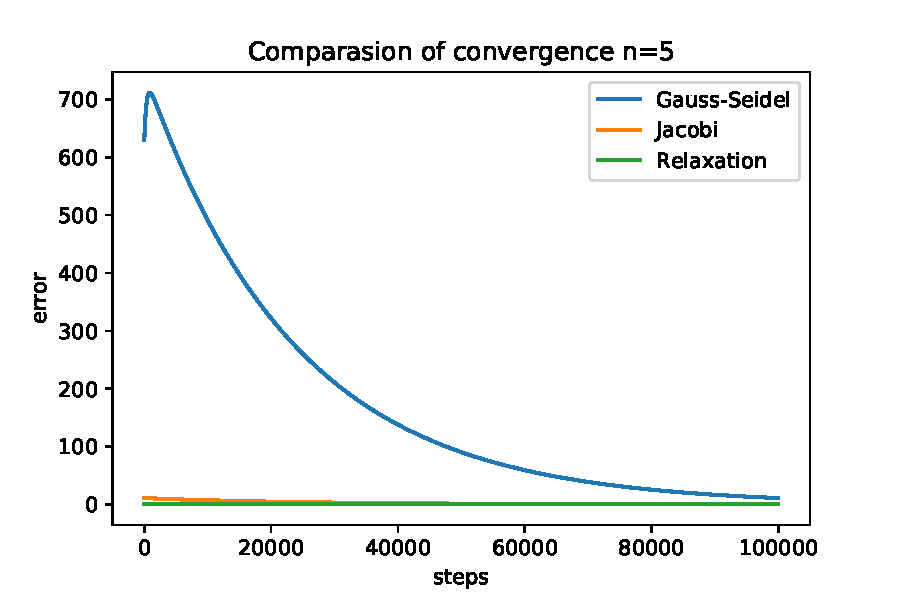
\includegraphics[]{n5-all}
  		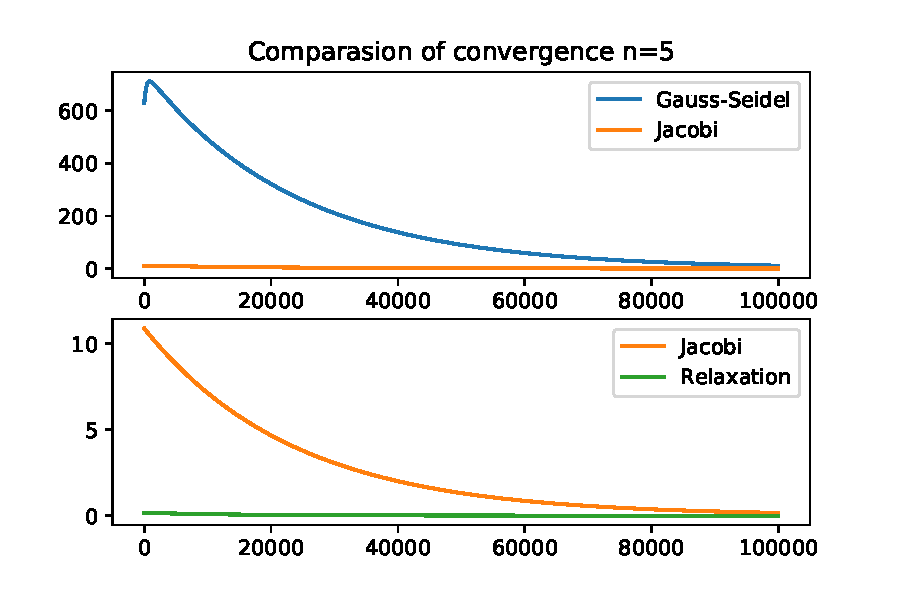
\includegraphics[]{n5}  
    \end{figure}		
  	
    \begin{figure}
    	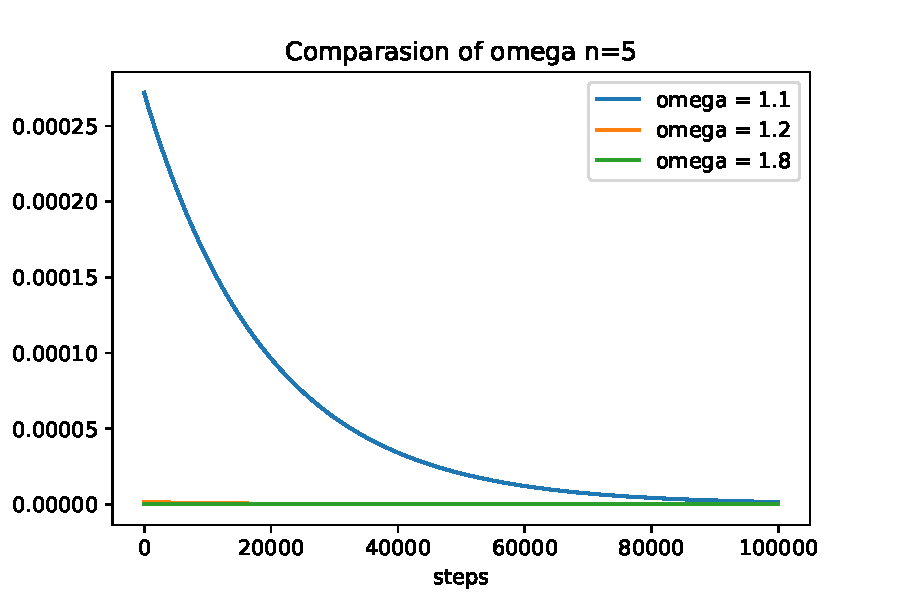
\includegraphics[]{omega-n5}
  		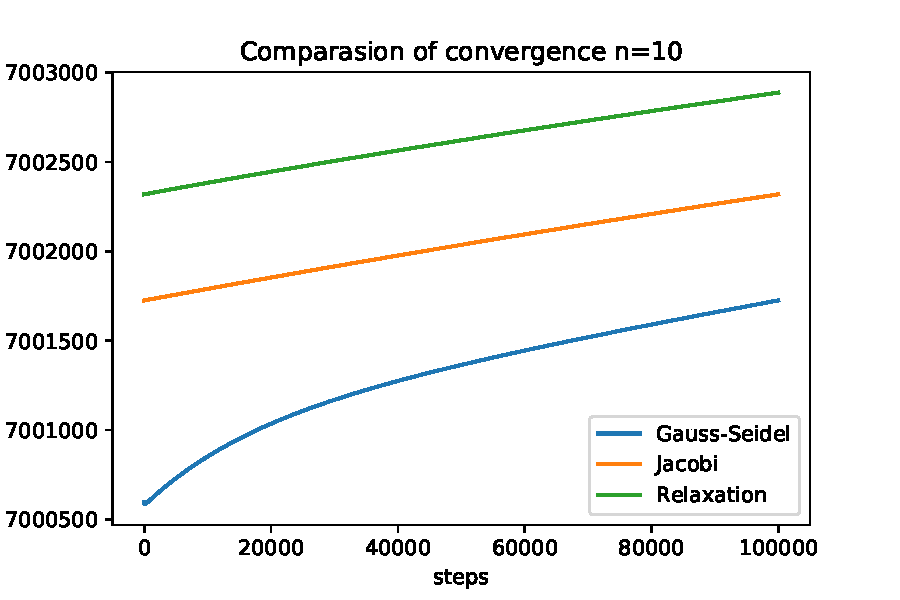
\includegraphics[]{n10-all}
  	\end{figure}
  	\begin{figure}
  		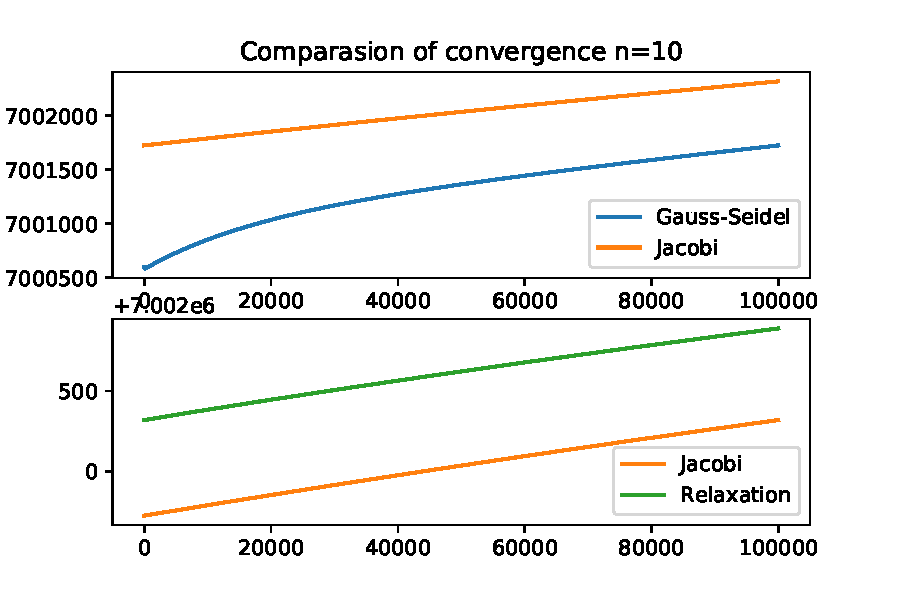
\includegraphics[]{n10}
  		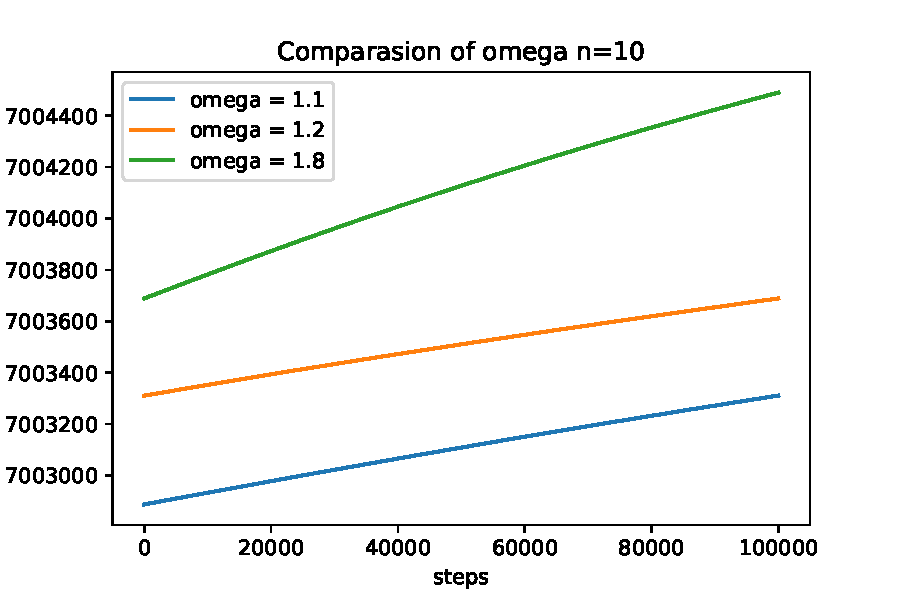
\includegraphics[]{omega-n10}
  	\end{figure}
  	
  \end{proof}  



\end{document} 